\documentclass[a4paper]{article}
\usepackage{cmap}
\usepackage{mathtext}
\usepackage{amssymb}
\usepackage{amsmath}
\usepackage[russian]{babel}
\usepackage{indentfirst}
\usepackage[pdftex]{graphicx}
\usepackage{multirow}
\usepackage{mathrsfs}
\usepackage{siunitx}
\usepackage[left=2cm,right=2cm,top=2cm,bottom=2cm]{geometry}
\usepackage{fancyhdr}
\pagestyle{fancy}
\newcommand{\rref}[1]{(\ref{#1})}
\newcommand{\mbf}{\mathbf}
\newcommand{\Equip}[3]{
	
	{\bf #1:} $\Delta = \pm #2$ \si{#3}}
\newcommand{\equip}[1]{
	
	{\bf #1}}
\newcommand{\labname}{Эффект Холла в полупроводниках.} 	% название пиши здесь
\newcommand{\labnum}{3.3.4.}										% номер вводи здесь
\fancyfoot{}
\fancyhead[RE, RO]{\thepage}
\fancyhead[LE, LO]{Лабораторная работа \labnum \space \labname}
\title{Лабораторная работа \labnum \space \labname} % Название работы здесь
\author{Иван Сладков}
\begin{document}
\maketitle
\thispagestyle{empty}
\section{Аннотация}
В данной работе проводится измерение подвижности и концентрации носителей заряда в полупроводниках посредством изучения зависимости ЭДС Холла от внешнего магнитного поля и тока, протекающего по образцу. Также изучается тип проводимости данного образца.

\section{Теоретические сведения}
Проводимость определяется формулой 
\begin{equation*}\label{проводимость}
	\sigma = e n b,
\end{equation*}
где $ n $ -- концентрация, а $ b $ -- подвижность носителей заряда (электронов и дырок).
Изучая эффект Холла, можно определить концентрацию; отсюда и подвижность.

Суть эффекта Холла состоит в появлении разности потенциалов между гранями проводника с током, помещённого в магнитное поле. На рисунке \ref{образец} ЭДС между гранями А и Б.
\begin{figure}[tb]
	\centering
	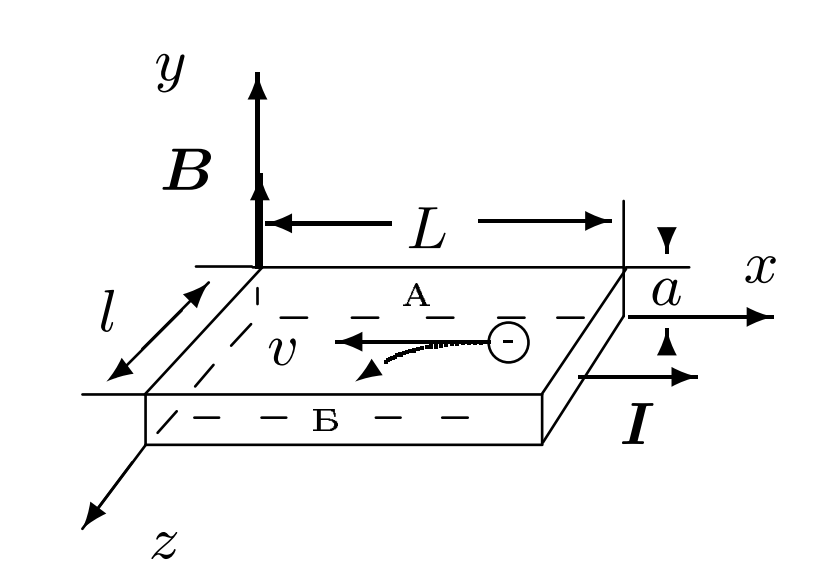
\includegraphics[width=0.8\linewidth]{образец}
	\caption{Образец с током в магнитном поле}
	\label{образец}
\end{figure}
В магнитном поле на электрон действует сила Лоренца:
\begin{equation*}\label{лоренц}
	{\mbf F}_Л = {\mbf F_E}+ {\mbf F_B} = e \mathbf{E}-e \left[\left<\mathbf{v}\right>, \mathbf{B}\right].
\end{equation*}
Здесь $ \mathbf{v} $ -- дрейфовая скорость электрона в электрическом поле. Под действием $ \mathbf{F_B} $ на торцах возникает ЭДС Холла. Бесконечному накоплению заряда на торцах препятствует $ F_{E z} = e E_z $. Из равенства её силе $ F_B $,
\begin{equation*}\label{key}
	E_z = \left|\left<v_x\right>\right| B.
\end{equation*}
Тогда 
\begin{equation*}\label{key}
	U_{А Б} = -E_z l = -\left|\left<v_x\right>\right| B l,
\end{equation*}
и окончательно для ЭДС Холла:
\begin{equation}\label{e}
	\mathscr{E} = U_{А Б} = -R_x \frac{I B}{a},
\end{equation}
\begin{equation}\label{key}
	R_x = \frac{1}{n e }.
\end{equation}
$ R_x $ -- постоянная Холла в металлах. В полупроводниках считаем, что превалирует один тип проводимости. Тогда это равенство верно.
\subsection{Расчётные формулы}

При расчёте калибровки магнита будет применяться формула
\begin{equation}\label{eq:calibre}
	B = \frac{Ф}{S N}.
\end{equation}

В основной части эксперимента будем использовать формулу \eqref{e}.

Удельную проводимость материала можно найти по формуле
\begin{equation}\label{key}
	\sigma = \frac{I L_{3 5}}{U_{3 5} a l},
\end{equation}
где $ L_{3 5} $ -- расстояние между контактами 3 и 5, $ a $ и $ l $ -- толщина и ширина образца.
\section{Оборудование и инструментальные погрешности}

\begin{figure}
	\centering
	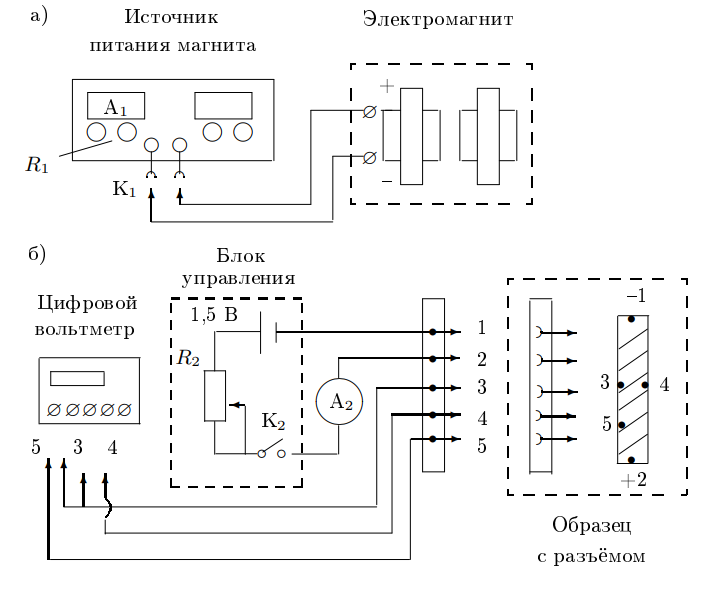
\includegraphics[width=0.8\linewidth]{схема}
	\caption{Схема экспериментальной установки}
	\label{fig:scheme}
\end{figure}

В эксперименте используется установка, изображённая на рис. \ref{fig:scheme}. В зазоре электромагнита создается постоянное магнитное поле, величину которого можно менять с помощью регуляторов источника питания электромагнита. Ток питания электромагнита измеряется амперметром источника питания. Градуировка магнита проводится при помощи измерителя магнитной индукции АТЕ-8702.
Образец из легированного германия, смонтированный в специальном держателе (рис. 16), подключается к батарее. При замыкании ключа вдоль длинной стороны образца течёт ток, величина которого регулируется реостатом и измеряется миллиамперметром.

Нужно заметить, что источник в ходе эксперимента выдавал достаточно низкий ток при максимальном напряжении. Причём со временем ток незначительно убывал ($\Delta I_{max} \simeq 0.01 $) А/ч. Это может быть связано, например, с нагревом катушки магнита.

\equip{Электромагнит}
\equip{Лабораторный источник питания}
\Equip{Амперметр на источнике}{0.01}{\ampere}
\Equip{Вольтметр на источнике}{0.1}{\volt}
\Equip{Вольтметр}{1}{\micro \volt}
\Equip{Миллиамперметр}{0.01}{\milli \ampere}
\Equip{Милливеберметр}{0.1}{\milli \weber}; $ S N = 75\; \left[ см^2 виток\right]  $

\equip{Реостат}
\equip{Батарейка}
\equip{Образец из легированного германия}: $ a = 2.2  $ мм, $ L_{3 5} = 6,0 $ мм, $ l = 7 $ мм.


\section{Результаты измерений и обработка данных}

\emph{Все измерения и расчёты в СИ.}

\subsection{Градуировка электромагнита}

По данным табл. \ref{tab:calibre} построим калибровочный график. 
\begin{table}
	\centering
\begin{tabular}{|l|l|l|l|}
	\hline
	$I_{mag},$ A & $Ф_1, мВб$, & $Ф_2, $мВб & $B$, Тл \\ \hline
	0            & 1.85        & 1.85       & 0.00    \\ \hline
	0.19         & 2.9         & 1.85       & 0.140   \\ \hline
	0.38         & 4           & 1.85       & 0.287   \\ \hline
	0.59         & 5.17        & 1.85       & 0.443   \\ \hline
	0.79         & 4.9         & 0.6        & 0.573   \\ \hline
	0.97         & 5.8         & 0.7        & 0.680   \\ \hline
	1.19         & 6.6         & 0.75       & 0.780   \\ \hline
	1.38         & 7.1         & 0.85       & 0.833   \\ \hline
	1.6          & 7.6         & 0.95       & 0.887   \\ \hline
\end{tabular}
	\caption{Данные для калибровки электромагнита}
	\label{tab:calibre}
\end{table}

\begin{figure}
	\centering
	\includegraphics[width=0.8\linewidth]{"калибровочный график"}
	\caption{Калибровочный график электромагнита}
	\label{fig:caibre}
\end{figure}

\subsection{Расчёт концентрации}

Снимем зависимость $ U_{3 4}(B) $ для разных токов через образец и покажем на графике \ref{fig:EDS}. Найдём угловые коэффициенты и внесём в таблицу \ref{tab:coeff}.

\begin{figure}
	\centering
	\includegraphics[width=0.8\linewidth]{"график ЭДС"}
	\caption{Семейство графиков $U_{3 4}(B) $ для разных токов в образце}
	\label{fig:EDS}
\end{figure}


\begin{table}
	\centering
\begin{tabular}{|l|l|l|l|l|}
	\hline
	$I$, мА               &           &          &      & $R^2$                    \\ \hline
	\multirow{2}{*}{0.26} & Intercept & 3.46E-5  & 6E-7 & \multirow{2}{*}{0.99673} \\ \cline{2-4}
	& Slope     & -1.15E-4 & 1E-6 &                          \\ \hline
	\multirow{2}{*}{0.30} & Intercept & 4.14E-5  & 6E-7 & \multirow{2}{*}{0.99612} \\ \cline{2-4}
	& Slope     & -1.35E-4 & 1E-6 &                          \\ \hline
	\multirow{2}{*}{0.40} & Intercept & 5.46E-5  & 6E-7 & \multirow{2}{*}{0.99613} \\ \cline{2-4}
	& Slope     & -1.79E-4 & 1E-6 &                          \\ \hline
	\multirow{2}{*}{0.60} & Intercept & 8.25E-5  & 6E-7 & \multirow{2}{*}{0.99634} \\ \cline{2-4}
	& Slope     & -2.64E-4 & 1E-6 &                          \\ \hline
	\multirow{2}{*}{0.70} & Intercept & 9.75E-5  & 6E-7 & \multirow{2}{*}{0.99565} \\ \cline{2-4}
	& Slope     & -3.15E-4 & 1E-6 &                          \\ \hline
	\multirow{2}{*}{0.80} & Intercept & 1.12E-4  & 6E-7 & \multirow{2}{*}{0.99552} \\ \cline{2-4}
	& Slope     & -3.60E-4 & 1E-6 &                          \\ \hline
	\multirow{2}{*}{0.90} & Intercept & 1.25E-4  & 6E-7 & \multirow{2}{*}{0.99508} \\ \cline{2-4}
	& Slope     & -4.04E-4 & 1E-6 &                          \\ \hline
\end{tabular}
	\caption{Коэффициенты прямых графика \ref{fig:EDS}}
	\label{tab:coeff}
\end{table}

По этим данным в свою очередь будем строить график зависимости $ K(I), $ где $ K = \frac{\mathrm{d} \mathscr{E}}{\mathrm{d} B} $ -- коэффициент наклона графиков \ref{fig:EDS}. Результат на рис. \ref{k}.

\begin{figure}
	\centering
	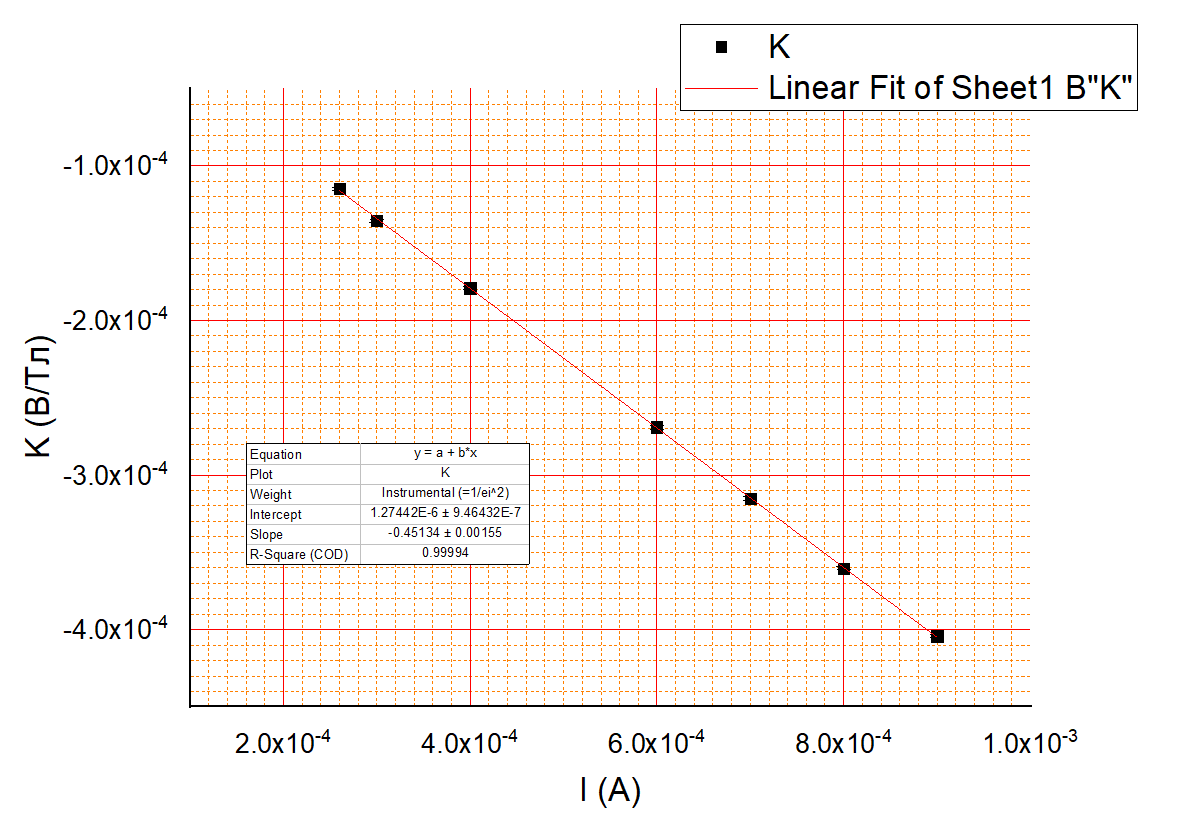
\includegraphics[width=0.8\linewidth]{k(I)}
	\caption{Зависимость K от тока в образце}
	\label{k}
\end{figure}

Т. к. $ K = -R_x I / a$, то $ \mathrm{d} K /\mathrm{d} I = -R_x / a $. 

\begin{equation}\label{5}
	R_x = - a \frac{\mathrm{d} K}{\mathrm{d} I} = 0.00099 \pm 1*10^{-5}\; м^3/Кл.
\end{equation}

Отсюда концентрация носителей заряда:

\begin{equation}\label{6}
	n = \frac{1}{e R_x} = 6.30*10^{21} \pm 2 * 10^{19}\; шт/м^3.
\end{equation}

Частицы -- электроны, т. к. при увеличении поля знак $ U_{3 4} $ становится <<->>. Схема на рис. \ref{fig:1}.

\begin{figure}
	\centering
	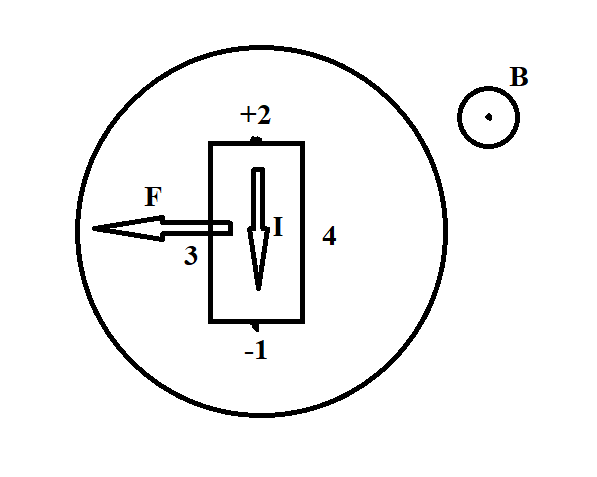
\includegraphics[width=0.8\linewidth]{1}
	\caption{Схема движения носителей заряда}
	\label{fig:1}
\end{figure}

\subsection{Расчёт удельной проводимости}

Для расчёта удельной проводимости материала сделали несколько замеров $ U_{3 5} $ и построили график \ref{fig:уд}, где
\begin{equation}\label{7}
	k = \lambda = \frac{\sigma a l}{L_{3 5}} = 0.406 \pm 0.001
\end{equation}

\begin{equation}\label{8}
	\sigma = \frac{\lambda L_{3 5}}{a l} = 184.5 \pm 0.5 \; Ом^{-1}.
\end{equation}

\begin{figure}
	\centering
	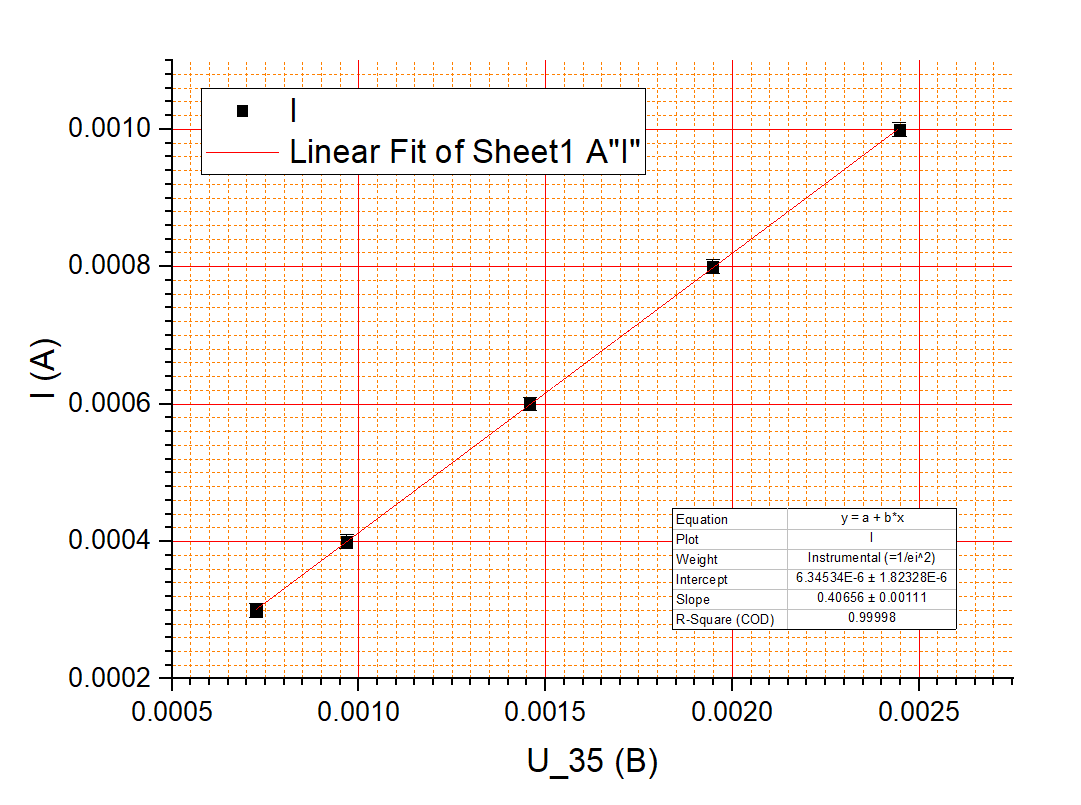
\includegraphics[width=0.8\linewidth]{удсопр}
	\caption{График для определения удельного сопротивления}
	\label{fig:уд}
\end{figure}


\subsection{Расчёт подвижности}

\begin{equation}\label{9}
	b = \frac{\sigma}{n e} = 0.183 \pm 0.001\; м^2/(В\; с) = 1830 \pm 10\; см^2/(В\; с)
\end{equation}

\subsection{Оценка погрешностей}

Погрешность формулы \eqref{eq:calibre} найдём следующим образом:
\begin{equation*}\label{key}
	\sigma_B = B \frac{\sqrt{2}\sigma_Ф}{(Ф_1- Ф_2)}.
\end{equation*}

Угловые коэффициенты и их погрешности во всех графиках находили в Origin. 

В формулах \eqref{5}, \eqref{6} пренебрегаем погрешностями $ a $ и $ e $ соответственно и находим погрешность:
\begin{equation*}\label{key}
	\sigma_{R_x} = R_x * \frac{\sigma_{d K/d I}}{d k/ d I}.
\end{equation*}

Аналогично в формулах \eqref{7} и \eqref{8}.

В \eqref{9} погрешность:

\begin{equation*}\label{key}
	\sigma_b = b \sqrt{\frac{\sigma_\sigma^2}{\sigma^2}+\frac{\sigma_n^2}{n^2}}
\end{equation*}

\section{Вывод}

Исследовав эффект Холла в полупроводниках, получили значения концентрации и подвижности свободных носителей. Выяснили, что это электроны. Нашли также удельную проводимость образца. 

Выполненные подсчёты очень приблизительны, т. к. реальная подвижность электронов в чистом германии $ \simeq 3700 \; см^2/(В\; с) $. Существенная неточность может быть связана с несовершенством эксперимента или с тем, что образец легирован, и поэтому подвижность отличается от табличной.
\begin{table}
	\centering
	\begin{tabular}{|l|l|l|l|l|}
		\hline
		$R_x, \; м^3/Кл$      & Знак носит. & $n, \; шт/м^3$     & $\sigma,\; (Ом/м)^{-1}$ & $b, \; см^2/(В с)$ \\ \hline
		$(990\pm 10)*10^{-6}$ & << -- >>     & $(630\pm 2)*10^{19}$ & $184.5\pm 0.5$          & $1830\pm 10$       \\ \hline
	\end{tabular}
	\caption{Таблица результатов}
	\label{tab:my-table}
\end{table}


\begin{thebibliography}{9}
	\bibitem{Siv} Сивухин Д. В. \emph{Общий курс физики. Том 3 Электричество и магнетизм}, 2004
	\bibitem{kirich} Кириченко Н.А. \emph{Электричество и магнетизм.}, 2011
	\bibitem{max} \emph{Лабораторный практикум по общей физике. В 3 томах. Том 2. Электричество и магнетизм: учебное пособие} под ред. А. В. Максимычева, М. Г. Никулина
\end{thebibliography}
\end{document}